\chapter{Методы неинвазивного исследования мозга}
С момента изобретения неизвазивных (т.е. не требующих хирургического вмешательства) методов исследования головного мозга, нейронауки совершили качественный скачок в знаниях о функциональном и структурном устройстве мозга. 
\section{Электроэнцефалография}
\indent Ранним методом неизвазивных исследований является электроэнцефалограмма (ЭЭГ), записывающая электрическую активность коры головного мозга. Однако этот метод является недостаточно точным и имеет много проблем – в первую очередь это зашумление данных, так как регистрация сигналов производится с помощью электродов, закрепленных на поверхности головы, и на сигнал оказывают большое влияние как физиологические факторы (между источником сигнала и электродами находится толстый слой тканей, в первую очередь, костной ткани черепа), так и человеческий фактор – в зависимости от расположения электродов на поверхности головы данные могут сильно варьироваться. Наибольшей проблемой является невозможность различить фактический вклад разных регионов, расположенных в глубине мозга, так как ЭЭГ регистрирует только поверхностную активность нейронов. Это ставит исследователей перед необходимостью решать задачу о «коктейльной вечеринке», в которой требуется из смеси большого количества сигналов точно отследить необходимые и определить их источники.
\section{Магнитно-резонансная томография}
Гораздо более точным методом исследования является магнитно-резонансная томография, основанная на измерении электромагнитного отклика атомных ядер веществ, содержащихся в головной мозге. Выделяют два основных вида магнитно-резонансной томографии:
\begin{itemize}
    \item Диффузионно-взвешенная МРТ
    \item Функциональная МРТ
\end{itemize}
\indent Диффузионно-взвешенная МРТ представляет собой метод измерения диффузии молекул воды в тканях мозга. Молекулярная дифузия в биологических тканях не является сводобной, на нее влияют множество препятствий, такие как макромолекулы, мембраны и волокнистые ткани. Паттерны диффузии позволяют различить микроскопические особенности устройства ткани, в том числе детектировать здоровые или пораженные заболеванием ткани. Особый вид дМРТ, диффузионно-тензорная томография, широко используется для исследования белого вещества мозга.\\
\indent Функциональная МРТ измеряет активность головного мозга с помощью замера изменений в потоке крови. Эта техника основана на том факте, что движение кровяных потоков и нейронная активность тесно связаны: если зона мозга активируется, то поток крови в ней становится сильнее. \\
\indent Оба вида томографии позволяют обойти ограничения, которые представляет ЭЭГ как метод исследования структуры и активности мозга: при съемке магнитно-резонансного изображения мозг анализируется в объеме, итоговые снимки представляют из себя трехмерное отображение структуры мозга (в случае структурной, диффузионно-взвешенной МРТ), либо четырехмерное отображение активности мозга (в случае функциональной МРТ; четвертым измерением является время). Также сильно снижено влияние человеческого фактора, поскольку для снятия МРТ-снимка человека полностью погружают в специально оборудованную машину – томограф.
\section{Коннектомика}
\indent В последнее время особую популярность приобрело представление структурного или функционального устройства мозга в виде взвешенного графа, в котором вершинами являются зоны мозга, а ребрами – структурные или функциональные связи между этими зонами. Такие графы называются коннектомами и являются полноценным описанием мозга и особенной его функционирования.Термин «коннектомика» появился в 2005 году и с тех пор приобрел широкую популярность в кругах исследователей, занимающихся задачами исследования нейроданных.\\
\indent Функциональные коннектомы строятся на основе снимков фМРТ, анализируя функциональные связи между регионами мозга, тогда как структурные коннектомы строятся по дМРТ и ребрами являются физиологические связи (нейронные тракты) между регионами мозга, а вес ребер зависит от количества трактов, проходящих между двумя зонами. \\
\newpage
\indent Коннектомы могут охватывать представления разных масштабов, от представления на макро-уровне до полноценной карты всех нейронов мозга живого существа. Глобальной целью коннектомики на сегодняшний день является построение максимально подробной карты человеческого мозга. 
На изображении ниже представлен пример коннектома (слева), построенного по диффузионно-тензорному МРТ, и трактография нейронной ткани (справа)

\begin{figure}[h!]
    \centering
    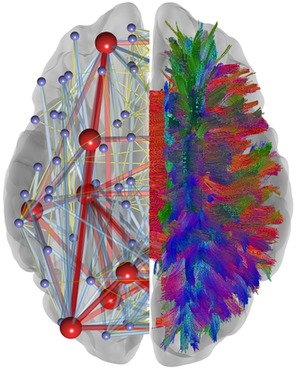
\includegraphics[width=0.5\textwidth]{img/connectome.jpg}
    \caption{Связи между зонами мозга, построенные на основе диффузионно-тензорной МРТ и трактографии нейронных тканей (справа). Коннектом, описывающий связи между зонами мозга. Многие виды нейродегенеративных заболеваний могут быть представлены как особенность подобных графов. \\ Изображение принадлежит Indiana University}
    \label{fig:my_label}
\end{figure}